\DocumentMetadata{}
\documentclass[sigconf, 10pt]{acmart}
\usepackage[compact]{titlesec}

\AtBeginDocument{%
  \providecommand\BibTeX{{%
    Bib\TeX}}}

\usepackage{hyperref}
\usepackage{longtable}
\usepackage{microtype}
\usepackage{enumitem}
\usepackage{xcolor}
\usepackage{amsmath,amsthm}
\usepackage{bbm}
\usepackage{subfigure}
\usepackage{graphicx}
\usepackage[font=small]{caption}
\usepackage{epstopdf}
\usepackage{algorithm}
\usepackage{tabularx}
\usepackage{multirow}
\usepackage[acronym,nogroupskip,nonumberlist,nopostdot]{glossaries}
\glsdisablehyper
\usepackage{xspace}
\usepackage{comment}
\usepackage{algorithm}
\usepackage[noend]{algorithmic}
\usepackage{makecell}
\usepackage{array}

\settopmatter{printacmref=false} % Removes citation information below abstract
\renewcommand\footnotetextcopyrightpermission[1]{} % removes 

\DeclareMathOperator*{\argmin}{arg\,min}
\DeclareMathOperator*{\argmax}{arg\,max}


\newcommand{\Expt}{\mathbb{E}}
\newcommand{\Prob}{\mathbb{P}}
\newcommand{\identity}{\mathbf{1}}
\newcommand{\Var}{\text{Var}}
\newcommand{\ttt}[1]{\texttt{#1}}
\newcommand{\cc}[1]{\mathcal{#1}}

\newcommand{\tblref}[1]{Table~\ref{#1}}
\newcommand{\equref}[1]{(\ref{#1})}
\newcommand{\figref}[1]{Fig. \ref{#1}}
\newcommand{\algref}[1]{Algorithm \ref{#1}}
\newcommand{\secref}[1]{Section \ref{#1}}
\newcommand{\appref}[1]{Appendix \ref{#1}~\cite{appendix}}
\newcommand{\lemmaref}[1]{Lemma \ref{#1}}
\newcommand{\defref}[1]{Definition \ref{#1}}
\newcommand{\exref}[1]{Example \ref{#1}}



\begin{document}

\acmYear{2024}\copyrightyear{2024}
\setcopyright{acmcopyright}
\acmConference[ACM MobiCom '25]{The 31th Annual International Conference On Mobile Computing And Networking}{November, 2025}{Hong Kong SAR, China}
\acmBooktitle{The 31th Annual International Conference On Mobile Computing And Networking (ACM MobiCom '25), November, 2025, Hong Kong SAR, China}
\acmDOI{10.1145/00000000}
\acmISBN{00000000}

\newcommand{\eg}{{\em e.g.}}

\newcolumntype{L}[1]{>{\raggedright\let\newline\\\arraybackslash\hspace{0pt}}m{#1}}
\newcolumntype{C}[1]{>{\centering\let\newline\\\arraybackslash\hspace{0pt}}m{#1}}
\newcolumntype{R}[1]{>{\raggedleft\let\newline\\\arraybackslash\hspace{0pt}}m{#1}}

\renewcommand{\cellalign}{vh}
\renewcommand{\theadalign}{vh}
\newcommand{\tsc}[1]{\textsuperscript{#1}}

\newtheorem*{takeaway*}{Takeaway}

\newcommand{\red}[1]{\textcolor{red}{#1}}

\newenvironment{sitemize}{
        \begin{list}{$\bullet$}{
                        \setlength{\itemsep}{2pt}
                        \setlength{\leftmargin}{1.2em}
                        \setlength{\topsep}{2pt plus 2pt minus 2pt}
                        \setlength{\parsep}{0.0cm}}
        }{\end{list}}

\newenvironment{senumerate}{
        \begin{list}{\arabic{enumi}.}{
                        \setlength\labelwidth{1.5em}
                        \setlength\leftmargin{1.5em}
                        \setlength{\topsep}{4pt plus 2pt minus 2pt}
                        \setlength\itemsep{0.0cm}
                        \usecounter{enumi}}
        }{\end{list}}

\settopmatter{authorsperrow=1}
\author{Changhan Ge}
\renewcommand{\shortauthors}{Changhan Ge}
\affiliation{
   \institution{The University of Texas at Austin, Austin, TX, USA}
   \institution{chge@utexas.edu}
   \country{}
   \city{}
}

\title{Petition for the Adoption of Year-specific Conference Branding Since ACM MobiCom 2025}

\newcommand{\wrt}{{\em w.r.t. }}
\newcommand{\para}[1]{\smallskip\noindent {\bf #1}}

\setlength{\abovecaptionskip}{0pt}
\setlength{\belowcaptionskip}{0pt}
\setlength{\abovedisplayshortskip}{0pt}
\setlength{\belowdisplayshortskip}{0pt}
\setlength{\textfloatsep}{0pt}

\begin{abstract}
This is a petition letter to the steering committee of the special interest group on mobile computing of association of computing machinery (hereinafter as SIGMOBILE), and the organizing committee of the 31st annual international conference on mobile computing and networking (hereinafter as ACM MobiCom 2025). Changhan Ge, a final year Ph.D. student at the University of Texas at Austin, the signer of this letter, sincerely hope the SIGMOBILE steering committee to adopt year-specific conference branding for all the conferences it sponsors, starting from ACM MobiCom 2025. A proposed logo for ACM MobiCom 2025 is submitted alongside the petition letter.
\end{abstract}

\keywords{MobiCom 2025, SIGMOBILE, Branding}

%\pagenumbering{gobble}

\settopmatter{printfolios=true}

\maketitle

\section{Petition}
In recent years, an increasing trend of using year-specific branding for academic conferences has been set off in the nearby academic communities, such as data communication community (\eg, SIGCOMM) and computer vision community (\eg, CVPR). Based on the discussions with peer scholars, we attribute this trend to the following reasons.
\begin{itemize}[leftmargin=*]
	\item Identity and Branding: A year-specific logo helps create a unique identity for each year's conference. It allows organizers to distinguish one edition from another while maintaining a consistent conference brand. This differentiation helps with the visual impact and makes each event memorable.
	
	\item Event Localization: By incorporating design elements that reflect the location or theme of that particular year, such as using local symbols or cultural icons, the logo connects the conference to its host city and gives it a local flavor. This fosters a sense of place and community, which is especially important for international conferences.
	
	\item Recognition and Legacy: Academic conferences often have a long history. Year-specific logos can help build a visual archive, creating a sense of legacy and continuity across years. This allows participants, researchers, and attendees to easily recognize which edition of the conference they are attending or discussing, even years later.
	
	\item Modern Aesthetic Appeal: Logos are part of modern design trends, and creating unique, year-specific logos reflects the evolving preferences of conference organizers and designers. These logos often incorporate dynamic, contemporary design elements, which appeal to younger, tech-savvy audiences.
	
	\item Sponsorship and Marketing: A year-specific logo is also a useful tool for sponsorship and marketing. It can be used on promotional materials, merchandise, websites, and social media, helping to create buzz and build anticipation for the event. It also provides flexibility in terms of how sponsors are visually represented with that year’s logo. This is specifically important for our SIGMOBILE community as the author witnesses a massive declining in conference sponsorship from industry. For your reference, ACM MobiHoc has already experienced 2 consecutive years of zero corporate sponsors, and MobiCom 24 has only 4 sponsors from industry (nearly 50\% reduction comparing with MobiCom 2019). Although it could be a result of weak market, we still see nearby academic community continues to draw industry's attention (\eg, SIGCOMM has 14 sponsors from industry)). As a Ph.D. student speaking on behalf of my peer students, this low interest from industry gives us a looming feeling in the job market in recent years. Although the marketing issue and industry-involvement should be saved for separate discussion, we still would like to bring steering committee's attention on this issue in this petition letter.
	
	\item Thematic Focus: In some cases, the conference theme might change yearly, and the logo can be designed to reflect that theme. This allows attendees to immediately grasp the primary focus of that year’s event, such as specific technological advancements or research areas.
\end{itemize}
To sum up, adopting a year-specific conference logo has become essential in today's competitive academic and professional environment. As conferences grow in scale and global participation, a unique logo for each edition helps distinguish one event from another, fostering a stronger identity and recognition. This approach not only captures the distinct theme, location, or focus of the conference but also enhances its branding, making it more memorable for attendees, sponsors, and the broader academic community. A year-specific logo can be used across promotional materials, websites, and social media, creating consistency and excitement around the event. Moreover, it allows conferences to visually connect with their host cities or regions, making the event feel more localized and culturally relevant. In an era where digital presence and visual impact are crucial, adopting such logos is a powerful tool to build engagement, maintain continuity across years, and ensure that each edition stands out. For these reasons, the urgency to adopt year-specific logos is undeniable, as it strengthens both the conference's legacy and its connection to a global audience. For your reference, we've attached the branding designs from nearby academic communities in recent years in Appendix A (Fig. \ref{fig:sigcomm25logo}, \ref{fig:sigcomm24logo}, \ref{fig:sigcomm23logo}, \ref{fig:cvpr25logo}, \ref{fig:cvpr24logo}).

\section{Logo Design for MobiCom 2025}
As a part of the petition, we deign a preliminary logo for organizing committee's  reference. As shown in Fig. \ref{fig:logo}, the proposed logo for ACM MobiCom 2025 prominently incorporates a design that to reflect the cultural and symbolic elements of Hong Kong. There are two main designing elements described as follow:
\begin{itemize}[leftmargin=*]
	\item \textbf{Bauhinia Flower (Hong Kong’s Emblem):} The emblem of Hong Kong features a Bauhinia flower, which is often used to symbolize Hong Kong’s cultural significance and local heritage. We incorporate it by replacing the "0" in conference year "2025" with a modified version of the emblem. Specifically, we use pink and blush to recolor the originally maroon emblem, hence to reflect our young and vibrant community.
	
	\item \textbf{Victoria Harbour:} Victoria Harbour is one of Hong Kong’s most famous and iconic landmarks. The logo integrates elements that resemble the harbor, such as a wave-like pattern, a silhouette of ships, and the water itself, representing the flow of communication, global connectivity, and the idea of crossing boundaries. Victoria Harbour is also a hub of trade and technology, which aligns well with the themes of the conference focusing on mobile computing, networking, and beyond.
\end{itemize}
Note that, the silhouette of Hong Kong cityline  was designed with the help of ChatGPT, an LLM model owned and designed by OpenAI. The U.S. Copyright Office has already stated that works created by non-humans cannot be copyrighted \cite{copyright}. Hence there is no copyright issue involved in this logo design. The organizing committee and anyone who attend or involves in the conference can use the logo with no restrictions, free-of-charge, for non-profit purposes. To align with the ACM open-access initiative, and as per ACM President Yannis Ioannidis addressed at MobiCom '24 about "reaching a real democratic academic community", we open-source the logo at \cite{logo} and welcome anyone to try our design.

\begin{figure}[h]
	
	\centering
	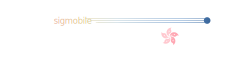
\includegraphics[width=\columnwidth, clip=true, trim=2cm 3cm 2cm 4cm]{../logo/mobicom25_logo.pdf}
	\caption{Proposed ACM MobiCom 2025 Logo}
	\label{fig:logo}
\end{figure}

\section {About the Designer}
Changhan Ge is a final year Ph.D. student in Computer Science at the Wireless Networking and Communications Group (WNCG) of The University of Texas at Austin, advised by Prof. Lili Qiu and Prof. Sanjay Shakkottai. His research interests mainly lie in wireless networking and mobile computing. Before he entered UT, he received his Master of Science in Electrical Engineering (Communication Theory and Systems) from the University of California San Diego (UCSD) in 2020, where he was fortunate to serve as a research assistant at the wireless networking group guided by Prof. Xinyu Zhang. Prior to that, he received his Bachelor of Engineering with honor in Network Engineering from the University of Electronic Science and Technology of China (UESTC) in 2018. 

Changhan Ge was also with AT\&T Labs in Bedminster NJ for the summer of 2022, 2023 and 2024 as a research intern working on analytics and automation of next-generation cellular network. During his time there, he was advised by Dr. Ajay Mahimkar and Dr. Zihui Ge.

\vspace{-3pt}
\section*{Acknowledgements}
\vspace{-3pt}
The author Changhan Ge @ UT Austin sincerely appreciates the help from ChatGPT, an LLM model owned and designed by OpenAI.

\appendix
\section{Logo Designs by Nearby Academic Community}
\begin{figure}[h]
	\centering
	\includegraphics[width=\columnwidth]{./appendix/sigcomm25-logo.png}
	\caption{SIGCOMM 2025 Logo}
	\label{fig:sigcomm25logo}
\end{figure}

\begin{figure}[h]
	\centering
	\includegraphics[width=\columnwidth]{./appendix/sigcomm24-logo.png}
	\caption{SIGCOMM 2024 Logo}
	\label{fig:sigcomm24logo}
\end{figure}

\begin{figure}[h]
	\centering
	\includegraphics[width=\columnwidth]{./appendix/sigcomm23-logo.png}
	\caption{SIGCOMM 2023 Logo}
	\label{fig:sigcomm23logo}
\end{figure}

\begin{figure}[h]
	\centering
	\includegraphics[width=\columnwidth]{./appendix/cvpr25-logo.jpg}
	\caption{CVPR 2025 Logo}
	\label{fig:cvpr25logo}
\end{figure}

\begin{figure}[h]
	\centering
	\includegraphics[width=\columnwidth]{./appendix/cvpr24-logo.png}
	\caption{CVPR 2024 Logo}
	\label{fig:cvpr24logo}
\end{figure}



\vspace{-3pt}
\bibliographystyle{ACM-Reference-Format}
\bibliography{reference}
\end{document}